% questions.tex —— 1962 年·全国卷 · 题目内容片段（无答案）
% 由 tools/generate_projects.py 依来源总账自 1962/1962_数学真题_试题.md 生成，勿手改（改源 MD 后重跑）


\begin{gktip}
\textbf{题面说明}：原卷要求只写题号，本文按题号 1—10 整理。原 PDF 第 1—5 页为 1962 年试题及答案，第 6 页已进入 1963 年试题，故不作为 1962 年题面。原卷答案页出现的图形在本库成品中以 TikZ 矢量源重绘。
\end{gktip}

\gkpart{一、小题}

\begin{question}
\gkti{1}某工厂第三年的产量比第一年的产量增长 $21\%$。问平均每年比上一年增长百分之几？又第一年的产量是第三年的产量的百分之几？（精确到 $1\%$。）

\end{question}
\begin{question}
\gkti{2}求 $(1-2i)^5$ 的实部。

\end{question}
\begin{question}
\gkti{3}解方程：

\[
\log(x-5)+\log(x+3)-2\log2=\log(2x-9)
\]

\end{question}
\begin{question}
\gkti{4}求

\[
\sin\left(2\arcsin\frac45\right)
\]

的值。

\end{question}
\gkpart{二、大题}

\begin{question}
\gkti{5}求证：

（1）圆内接平行四边形是矩形；

（2）圆外切平行四边形是菱形。

\end{question}
\begin{question}
\gkti{6}解方程组：

\[
\begin{cases}
y^2-4x-2y+1=0,\\
y=x+a
\end{cases}
\]

并讨论：$a$ 取哪些实数值时，这个方程组

（1）有不同的两组实数解；

（2）有相同的两组实数解；

（3）没有实数解。

\Needspace{0.4\textheight}
\end{question}
\begin{question}
\gkti{7}如图，$ABCD$ 和 $A'B'C'D'$ 都是正方形，而 $A'$、$B'$、$C'$、$D'$ 顺次分别把 $AB$、$BC$、$CD$、$DA$ 分成 $m:n$，并设 $AB=1$。
\nopagebreak[4]
\begin{center}% 1962 年全国卷第 7 题：正方形边上按 m:n 分点形成内接正方形。
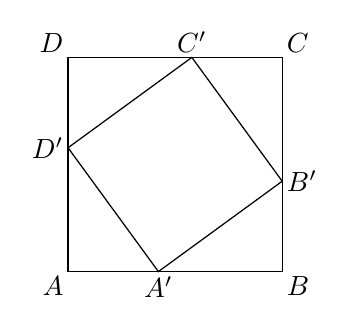
\begin{tikzpicture}[scale=0.85, line width=0.45pt,
  every node/.style={inner sep=1.5pt}]
  \coordinate (A) at (0,0);
  \coordinate (B) at (3.2,0);
  \coordinate (C) at (3.2,3.2);
  \coordinate (D) at (0,3.2);
  \coordinate (Ap) at (1.35,0);
  \coordinate (Bp) at (3.2,1.35);
  \coordinate (Cp) at (1.85,3.2);
  \coordinate (Dp) at (0,1.85);
  \draw (A)--(B)--(C)--(D)--cycle;
  \draw (Ap)--(Bp)--(Cp)--(Dp)--cycle;
  \node[anchor=north east] at (A) {$A$};
  \node[anchor=north west] at (B) {$B$};
  \node[anchor=south west] at (C) {$C$};
  \node[anchor=south east] at (D) {$D$};
  \node[anchor=north] at (Ap) {$A'$};
  \node[anchor=west] at (Bp) {$B'$};
  \node[anchor=south] at (Cp) {$C'$};
  \node[anchor=east] at (Dp) {$D'$};
\end{tikzpicture}
\end{center}
\nopagebreak[4]
（1）求正方形 $A'B'C'D'$ 的面积；

（2）证明：正方形 $A'B'C'D'$ 的面积不小于 $\dfrac12$。

\end{question}
\begin{question}
\gkti{8}$D$ 是 $\triangle ABC$ 内的一点，已知

\[
AB=AC=1,\qquad \angle CAB=63^\circ,
\qquad \angle DAB=33^\circ,\qquad \angle DBA=27^\circ,
\]

求 $CD$。（$\sin27^\circ=0.4540$。最后结果计算到小数点后两位。）

\end{question}
\begin{question}
\gkti{9}由正方体 $ABCD-A_1B_1C_1D_1$ 的顶点 $A$ 作这个正方体的对角线 $A_1C$ 的垂线，垂足为 $E$。证明：

\[
A_1E:EC=1:2
\]

（要求画图。）

\end{question}
\begin{question}
\gkti{10}求证：两两相交而不通过同一点的四条直线必在同一平面内。

\end{question}